
%%% Uncomment for slide version
\documentclass{beamer}
\setbeameroption{hide notes} % Only slides

%%% Uncomment for handout version
%\documentclass[handout]{beamer}
%\setbeameroption{show notes on second screen=right} % Both


\usepackage{listings}
\usepackage{adjustbox}
\usepackage{multirow}

\setbeamertemplate{note page}{\pagecolor{white}\insertnote}
\setbeamertemplate{footline}{}
\usetheme[progressbar=frametitle]{moloch}% modern fork of the metropolis theme
\setbeamercolor{background canvas}{bg=white}
\setbeamercolor{progress bar}{use=palette primary,fg=red,bg=red}
\setbeamercolor{note page}{bg=white} 
\setbeamertemplate{date}{}





\defbeamertemplate*{title page}{customized}[1][]
{
	\usebeamerfont{title}\inserttitle\par
	\bigskip
	\bigskip
		\bigskip
			\bigskip

	\usebeamerfont{title}\usebeamercolor[fg]{subtitle}\insertsubtitle\par
	\bigskip
	\usebeamerfont{author}\insertauthor\par
	\usebeamerfont{subtitle}\insertinstitute\par
	\usebeamercolor[fg]{titlegraphic}\inserttitlegraphic
}
\setbeamertemplate{page number in head/foot}{}


\addtobeamertemplate{navigation symbols}{}{%
	\usebeamerfont{footline}%
	\usebeamercolor[fg]{footline}%
	\hspace{1em}%
	\insertframenumber/\inserttotalframenumber
}
\setbeamercolor{itemize item}{fg=black}
\setbeamercolor{itemize subitem}{fg=black}
\setbeamercolor{itemize subsubitem}{fg=black}

\newcommand\blfootnote[1]{%
	\begingroup
	\renewcommand\thefootnote{}\footnote{#1}%
	\addtocounter{footnote}{-1}%
	\endgroup
}


%%%%%%%%%%%%%%%%%%
%%%%%%%%%%%%%%%%%%
%%%%%%%%%%%%%%%%%%
%%%%%%%%%%%%%%%%%%
%%%%%%%%%%%%%%%%%%
%%%%%%%%%%%%%%%%%%
%%%%%%%%%%%%%%%%%%




\title{\Huge FRST302: Forest Genetics}
\author{\Large Lecture 1.1: Classical Genetics and its Molecular Mechanisms}
\date{\today}

\begin{document}
	\maketitle

\note{\emph{Remember, everything on the lecture slides and the accompanying notes is potentially examinable!}}
% for the beamer version
%\documentclass{beamer}


%%% Slide 2
	
\begin{frame}
		\frametitle{Outline for Today}
\setbeamertemplate{itemize items}[circle]
\Large{
			\begin{itemize} 
			\item Short history of genetics
			\item Mendel's laws
			\item Chromosomes
		\end{itemize}
	}

\note{
Learning Outcomes
	\emph{		\begin{itemize} 
				\item Basic definitions in genetics
				\item Principles and terms in classical genetics
				\item Molecular mechanisms of classical genetics
				\item Chromosome crossover and its significance
			\end{itemize}
	}
}
\end{frame}

%%% Slide 3
\begin{frame}
\frametitle{History of Genetics}

\Large \textbf{What is genetics?} \par

\bigskip
\pause
\Large \textbf{Genetics is the study of genes}, of variation and heredity across all branches of the tree of life




\end{frame}



%%% Slide 4

\begin{frame}
	
	\Huge \centering \emph{What are the major questions in genetics?}
	\vspace{20pt}
	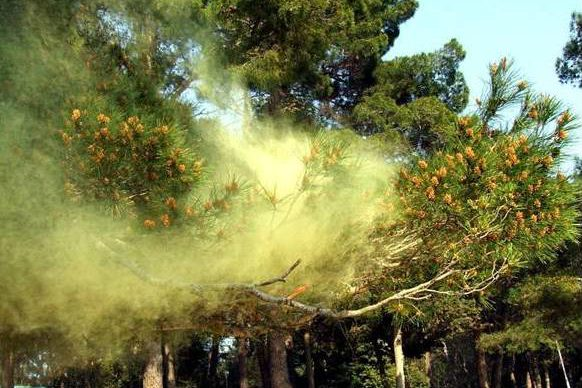
\includegraphics[keepaspectratio, width  =0.8\textwidth]{img/pollenPlume}
	\note{
		The answer to this question totally depends on your perspective. However, I think that it is more than fair to say that the following questions are at the heart of most biological science:
		\begin{itemize} 
			\item Why is there so much variation among individuals?
			\item How is this variation maintained in populations?
			\item Why do offspring tend to resemble their parents? 
			\par
		\end{itemize}
		
		\footnote \url{https://www.asthmacenter.com/wp-content/uploads/Pine-Pollen-Plume-e1495119706845.jpg}
	}
\end{frame}

%%% Slide 5
\begin{frame}
	
	How can we apply a knowledge of genetics?
	
	\vspace{5pt}
	
	\centering
	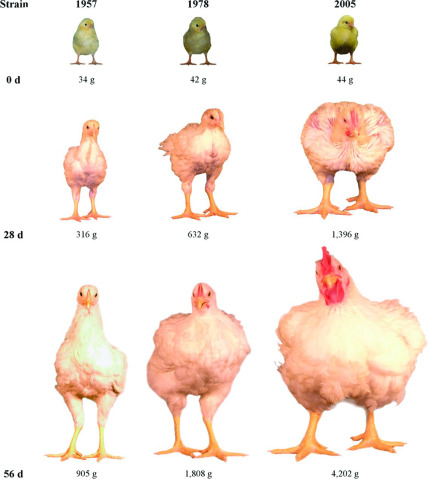
\includegraphics[keepaspectratio, width  =0.6\textwidth]{img/zuidhof_2014} \footnote {Modified from Figure 1 - Zuidhof et al. 2014}
\end{frame}

%%% Slide 6
\begin{frame}
	\frametitle{History of Genetics}
	
\begin{columns}[T]
	\begin{column}{.7\textwidth}
			Humans have probably pondered inheritence for all history:
			\vspace{10pt}
			\begin{itemize}
				\item For much of history, the mechanisms of inheritence were basically unknown
				\item The inheritance of acquired characteristics was widely accepted for much of history (from Hippocrates to Aristotal to Lamarck) \pause
				\item \emph{Early microscopists thought that they had seen small humans inhabiting sperm cells!}
			\end{itemize}
	\end{column}
	\begin{column}{.3\textwidth}
			% Your image included here
% TODO: \usepackage{graphicx} required
\centering
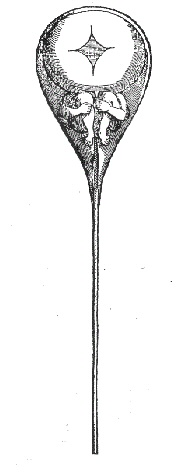
\includegraphics[keepaspectratio, width  = 0.8\textwidth]{img/homunculous}\footnotemark[1]


	\end{column}
\end{columns}
   \note{
	The inheritance of acquired characteristics is often referred to simply as Lamarkism after Jean-Baptiste Lamarck.

	Lamarck was an 19th century evolutionary biologist who formalised a lot of the contemporary thought on how biodiversity originated. The classic example is a giraffe stretching up to reach higher leaves would likely give birth to offspring with longer necks.
	
	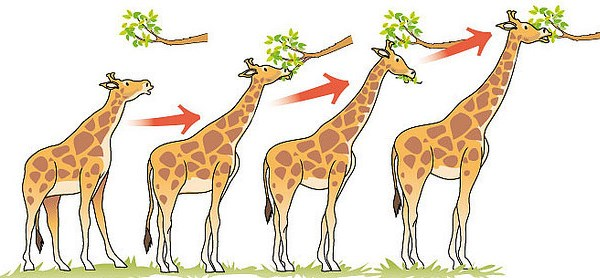
\includegraphics[keepaspectratio, width  = 0.8\textwidth]{img/lamarck}\\
			\url{https://simple.wikipedia.org/wiki/Lamarckism}
}
\end{frame}


%%% Slide 7
\begin{frame}
	\frametitle{History of Genetics}
	
	\begin{columns}[T]
		\begin{column}{.6\textwidth}
			By the 19th Century, the dominant theory was \textbf{blending inheritance}
		
			\vspace{5pt}
			\begin{itemize}
				\item The notion that an offspring's traits are simply the average of the parents' traits. 
				\item This is intuitively appealing -  continuously varying traits are often intermediate between their parents 
				\item \textit{There is one big problem with blending inheritance!}
			\end{itemize}
		\end{column}
		\begin{column}{.3\textwidth}
				\centering
			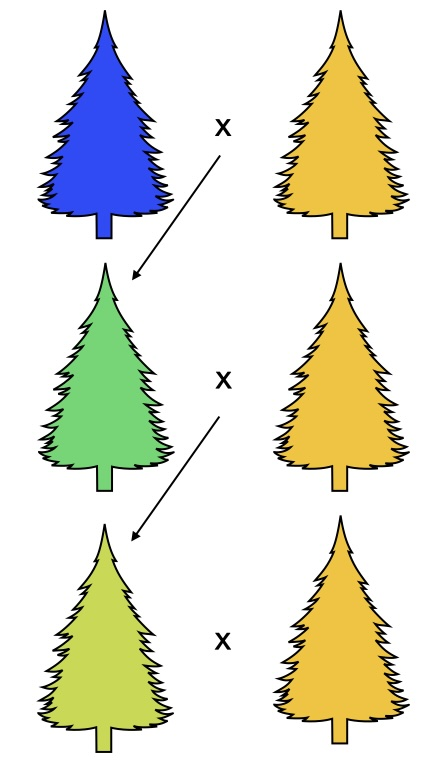
\includegraphics[keepaspectratio, width  = \textwidth]{img/blending}
		\end{column}
	\end{columns}
	

\end{frame}
	%%% Slide 8
\begin{frame}
		\frametitle{The Problem with Blending}
		
				\Huge \centering \emph{What's the big problem with blending inheritance?}
		   \note{
		   	The halving of variation each generation due to blending inheritance was first formalised by Fleeming Jenkin - the inventor of the cable car.\\
		   	Thus, under blending inheritance, half of the variation we see in natural populations at any given time would have to replenished each generation!
		   
		   }
\end{frame}




%%% Slide 9
\begin{frame}
	\frametitle{Darwin's Thoughts on Inheritance}
	\begin{columns}
		\begin{column}{0.5\textwidth}
			\small
			\textit{```The laws governing inheritence are quite unknown; no one can say why the peculiarity in different individuals of the same species... is sometimes inherited and sometimes not so"} \footnote[1]{\textit{Ch. 1, The Origin of Species, C. Darwin 1859}}
			
			\vspace{10pt}
			
			But, Darwin clearly appreciated the limitations of blending and felt the need for an alternative:
			
			\vspace{10pt}
			
			\textit{``Each parent transmits it peculiarities, therefore if varieties allowed to cross... such varieties will be constantly demolished" \footnote[2]{\textit{ Foundations of the `Origin of Species', F. Darwin 1909}}}
		\end{column}
		\begin{column}{0.4\textwidth}
			A NICE PIC OF DARWIN?
		\end{column}
	\end{columns}
	
	
	
\end{frame}


%%% Slide 9
\begin{frame}

	\frametitle{Trait Variation}

	Blending inheritence only really makes sense when you are thinking about continuously varying traits
	
	\vspace{5pt}

But different modes of variation are common:\pause
\begin{itemize}
	\item Continuous  - traits measured on a numerical scale (e.g. height, diameter, chlorophyll fluorescence) \pause
	\item Discrete - traits that exhibit categorical differences (e.g. different leaf forms, distinct flower colour) \pause
	\item Ordinal - discrete traits with some informative order (e.g. high, medium and low shade tolerance)
	
\end{itemize}

\end{frame}


%%% Slide 10
\begin{frame}
	
	\frametitle{Particulate Inheritance}
	
	\begin{columns}[T]
		
		\begin{column}{0.6\textwidth}
			
			Through careful experimentation analysing discrete traits in peas, Franciscan Friar Gregor Mendel found evidence supporting a model of particulate inheritence
			
			\vspace{10pt}
			
			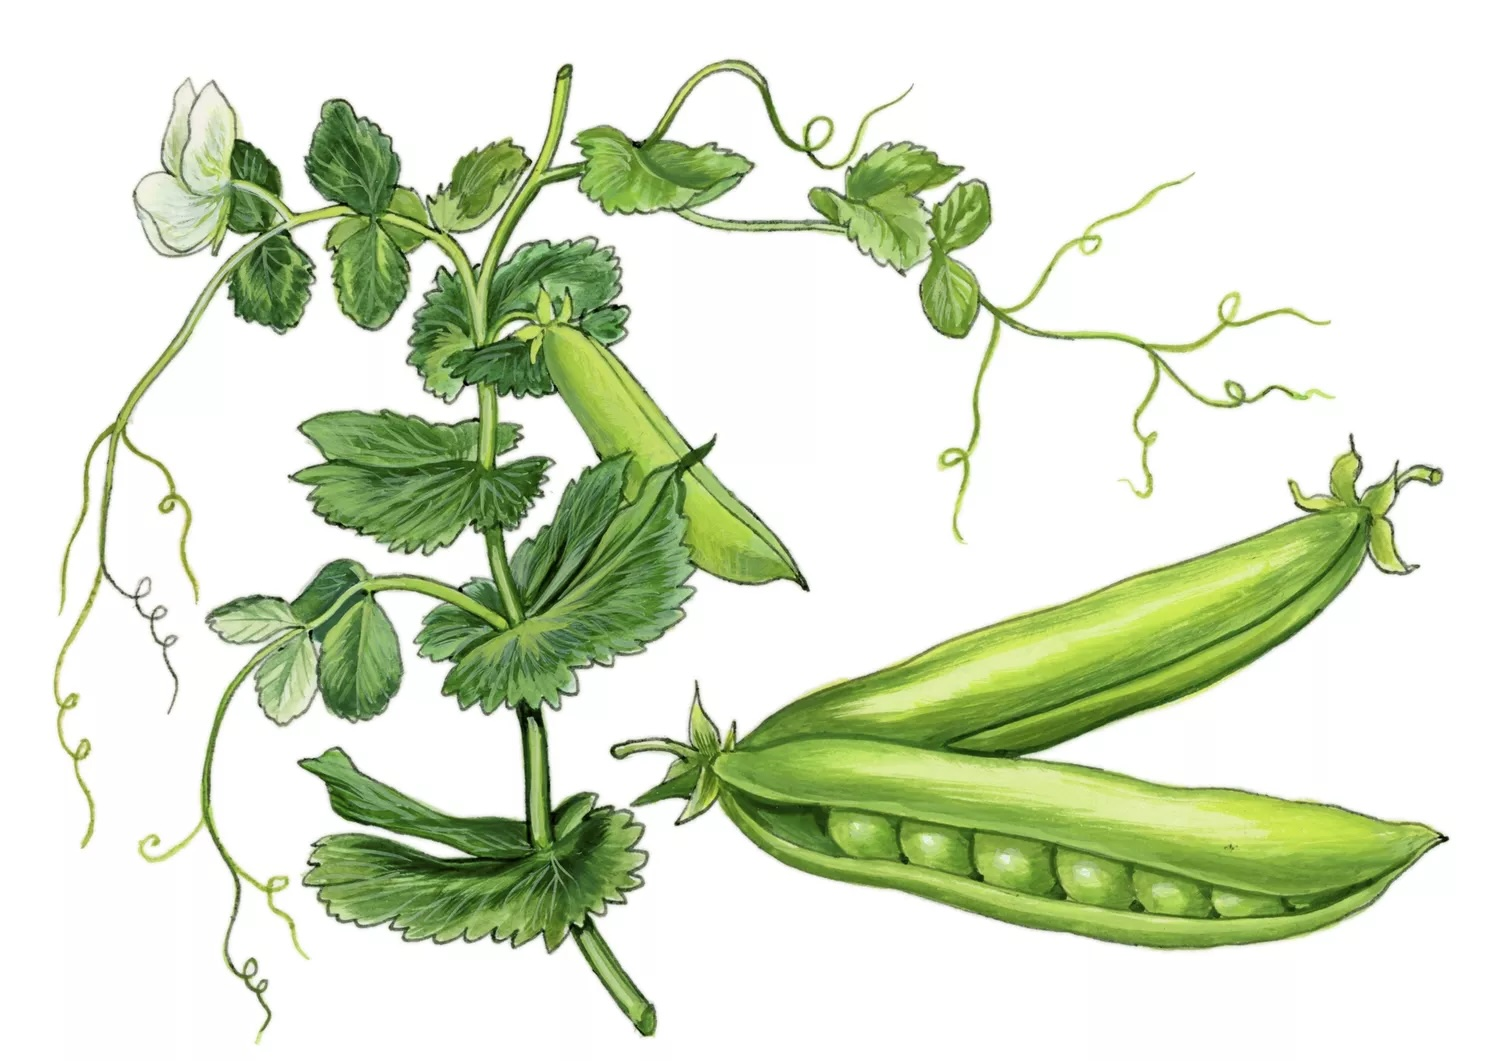
\includegraphics[keepaspectratio, width  =0.8\textwidth]{img/peas}

		\end{column}
		\begin{column}{.4\textwidth}
			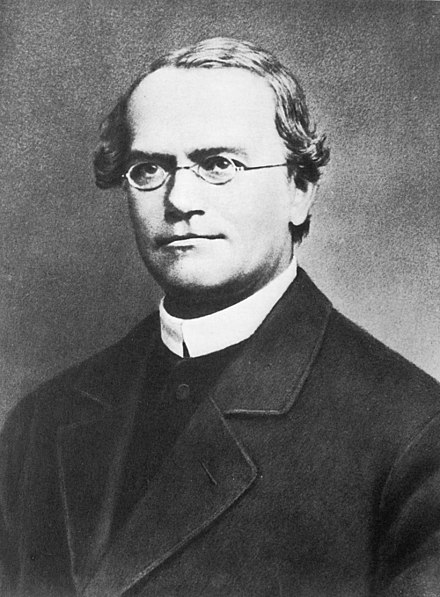
\includegraphics[keepaspectratio, width  =\textwidth]{img/mendel}
			\centering
			Mmmmm...\\
			Peas Peas Peas Peas Peas
		\end{column}
		
		\note{Pea pic from: \url{https://www.thoughtco.com/domestication-history-of-peas-169376}} 
	

		
	\end{columns}
\end{frame}


\begin{frame}
	
	\frametitle{Particulate Inheritance}
\textbf{Particulate Inheritance:} traits are passed from parent to offspring via particles \pause
\vspace{20pt}
\small
\begin{columns}
		\begin{column}{.5\textwidth}
			\underline{Blending Inheritance}
				\begin{itemize}
					\item{Offspring exhibit averages of parental traits}
					\item{The "blended" traits are transmitted to offspring}
					\item{Variation is rapidly lost across generations}
					
				\end{itemize}
			\end{column}
		\begin{column}{.5\textwidth}
			\underline{Particulate Inheritance}
				\begin{itemize}
					\item{Offspring exhibit  \textit{combinations} of parental traits}
					\item{Parental traits can manifest in offspring (or skip generations)}
					\item{Variation is maintained over time}					
				\end{itemize}
			\end{column}
	\end{columns}
	
\end{frame}



%%% Slide 11

\begin{frame}
	\frametitle{Mendel's Crosses}
	\centering
	Mendel examined variation and inheritence of several discrete characteristics of pea plants
	\vspace{10pt}

			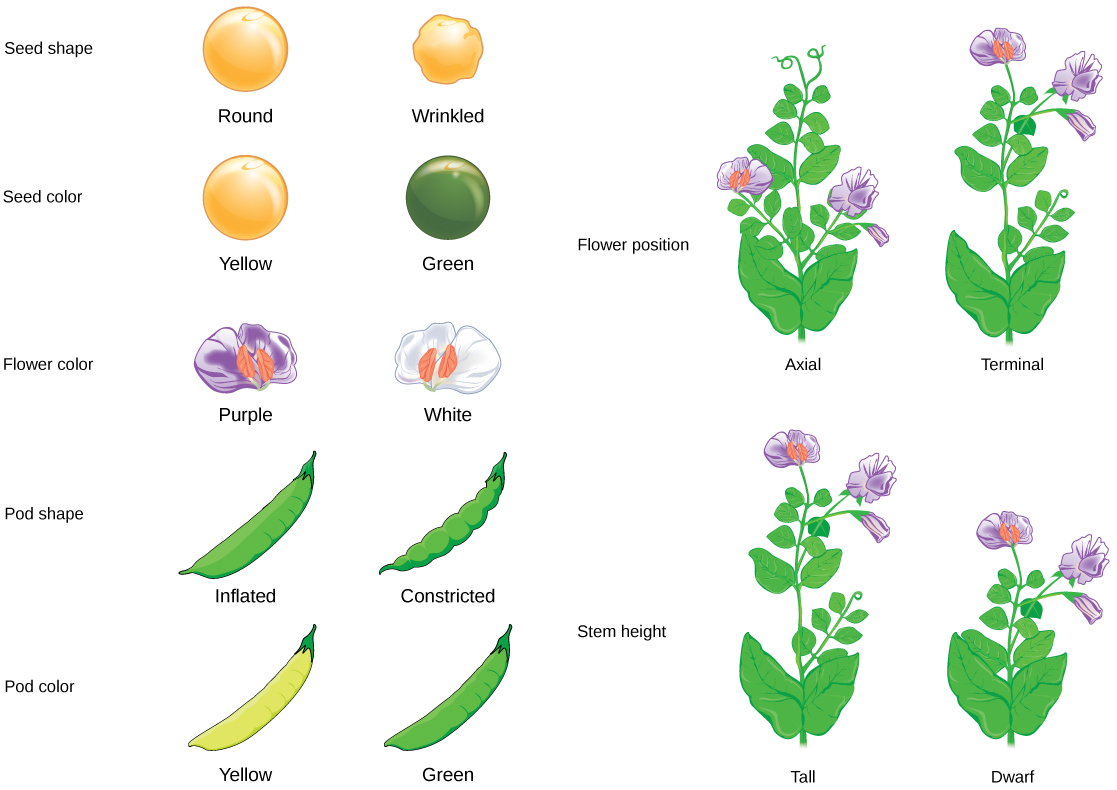
\includegraphics[keepaspectratio, width  =0.8\textwidth]{img/mendelCross_2}
\note{Figure from: \url{https://opentextbc.ca/biology/wp-content/uploads/sites/96/2015/02/Figure_08_01_03.jpg}}
\end{frame}
%%% Slide 12

\begin{frame}
	
	\frametitle{Mendel's Crosses}

	
\begin{columns}
	\begin{column}{0.5\textwidth}
			Garden peas are capable of self-fertilization, so Mendel was abel to generate "true" lines of peas that exhibit a particular trait/phenotype
		\begin{itemize}
	\item	Crossing lines produces an F1 generation \note{F1 stands for first filial generation. Subsequent crosses of individuals from the F1 generation will produce an F2, crossing individuals from the F2 generation will produce an F3 and so on...}	
	\item 	The patterns of variation among the F2 generations were Mendel's focus
		\end{itemize}
		


	\end{column}
	\begin{column}{0.6\textwidth}  
\begin{center}
			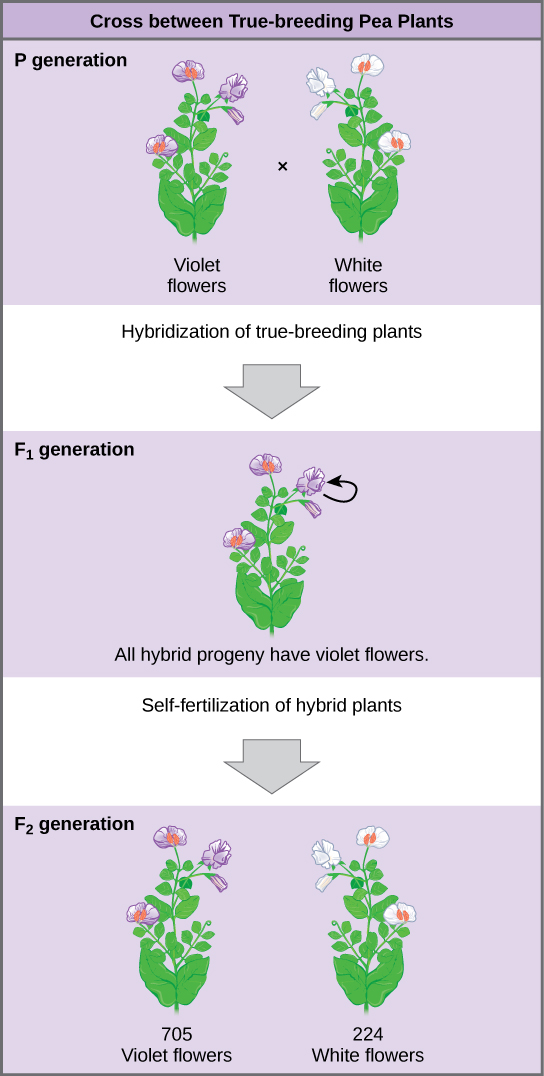
\includegraphics[keepaspectratio, width  =0.6\textwidth]{img/mendelCross_1}
\end{center}
\end{column}
\end{columns}
\end{frame}



\begin{frame}
	
	\frametitle{Mendel's Crosses}
\begin{center}
				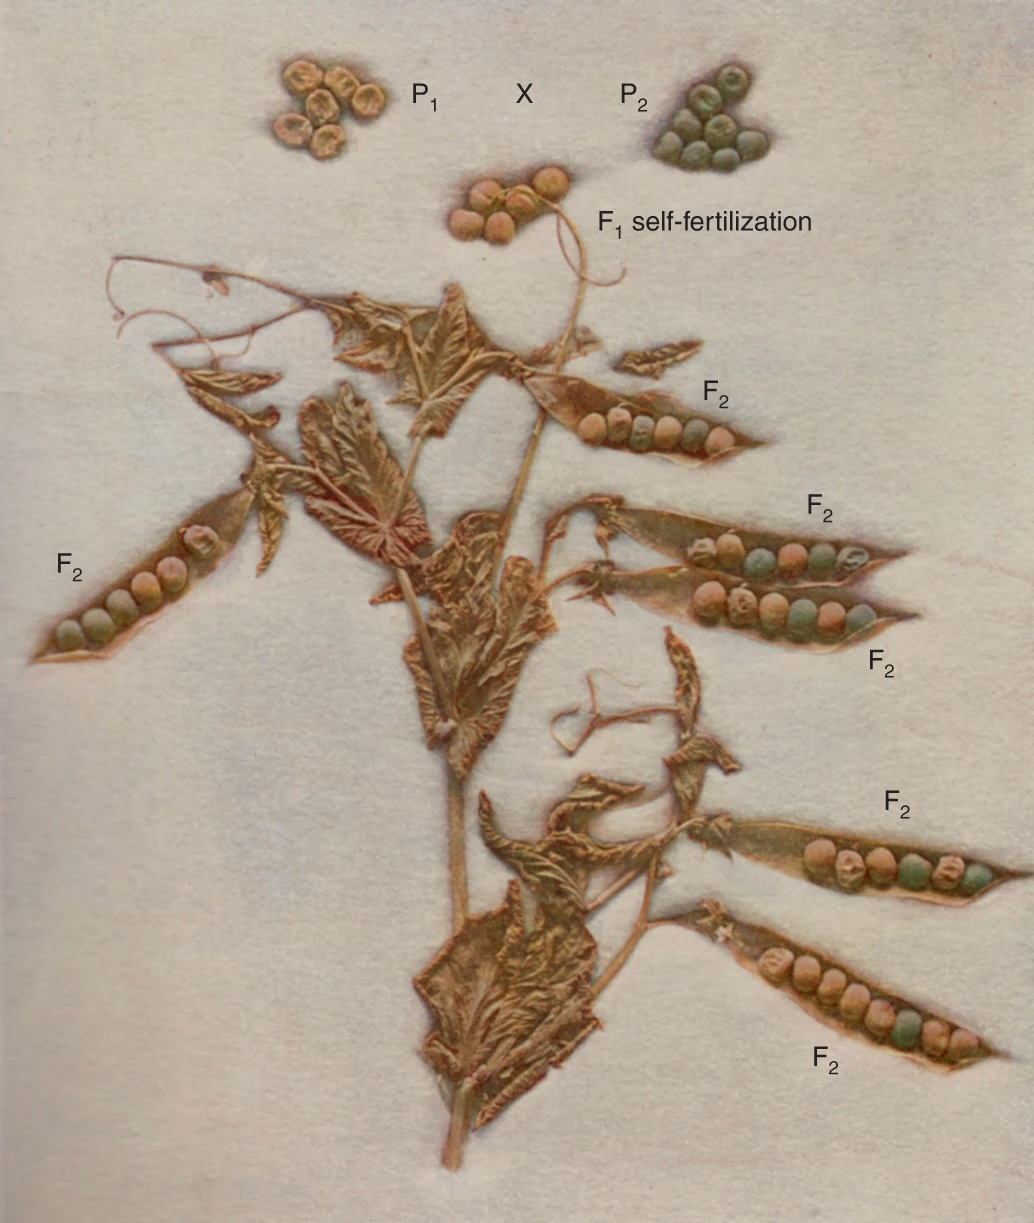
\includegraphics[keepaspectratio, width  =0.6\textwidth]{img/crossedPeas}
				\blfootnote{Note the 3:1 ratios of the two pea phenotypes in the F2}
\note{Figure 3 from: van Dijk, P.J., Jessop, A.P. \& Ellis, T.H.N. How did Mendel arrive at his discoveries?. Nat Genet 54, 926–933 (2022). https://doi.org/10.1038/s41588-022-01109-9}
	
	
\end{center}
\end{frame}


\begin{frame}
	
	\frametitle{Mendel's Laws}

The patterns of variation that Mendel observed led him to develop three laws of inheritance
\begin{itemize}
	\item Law of Segregation 
	\item Law of Dominance 
	\item Law of Independent Assortment
		\end{itemize}
	\end{frame}



%%% Slide 14


\begin{frame}
	\frametitle{Mendel's Laws}
	\textbf{The law of segregation: } each individual possesses a pair of particles for any particular trait and each parent passes one of these randomly to its offspring 

	\vspace{10pt}

		\textbf{The law of dominance: } for some traits, the presence of one kind of particle masks the presence of another. Mendel referred to the \textbf{dominant} particle as masking the effects of the \textbf{recessive} particle \pause
		
	\vspace{10pt}
		
			\textbf{The law of independant assortment:} when two individuals differ in more than two pairs of traits (e.g. smooth v. wrinkly and green v. yellow), the inheritance of one pair of traits is independent of another 
		
\end{frame}



\begin{frame}
	
	\frametitle{Mendel's Laws}
	\begin{columns}
	\begin{column}{0.6\textwidth}
		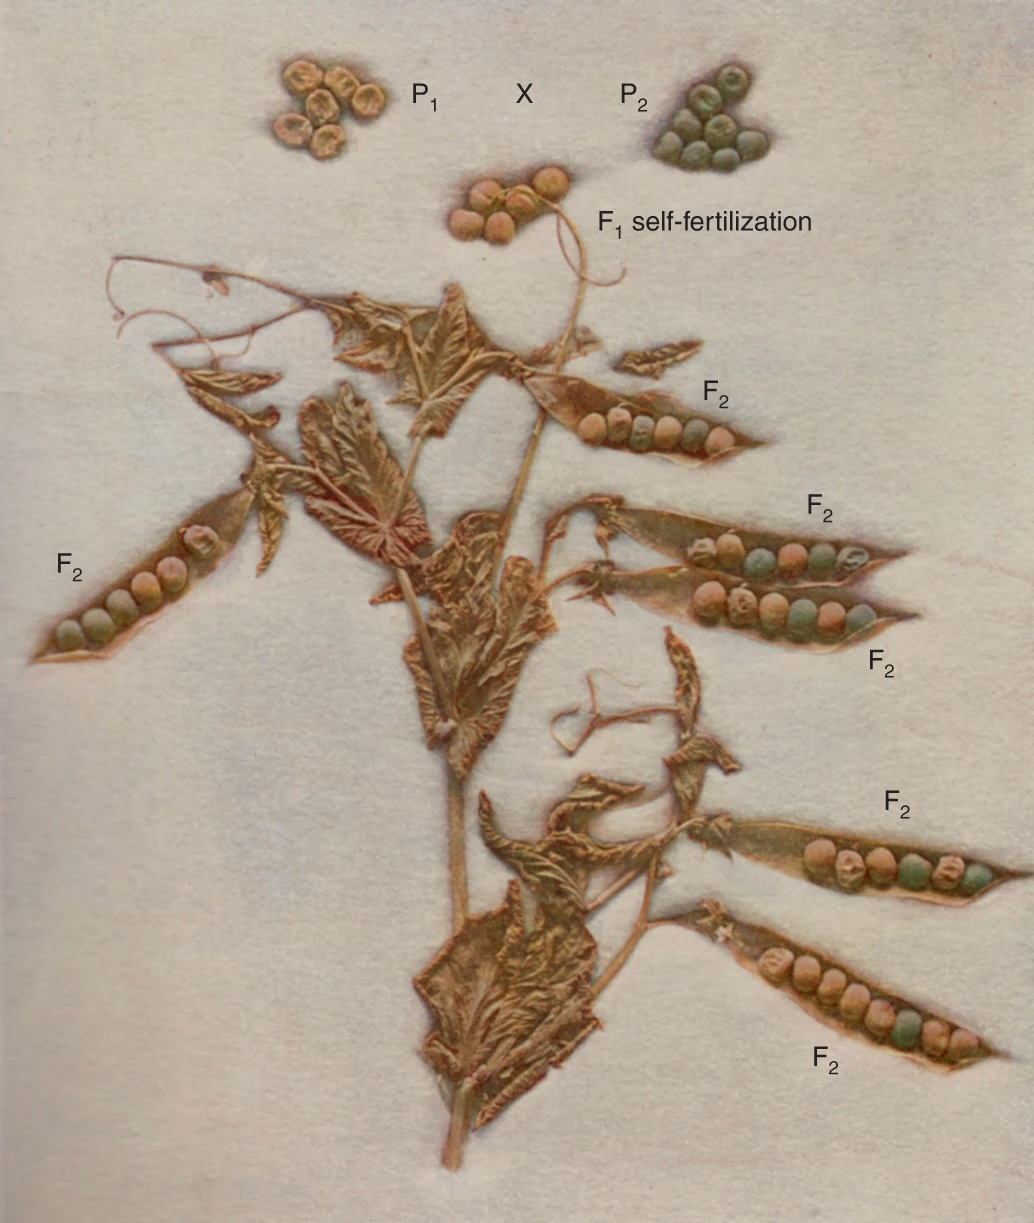
\includegraphics[keepaspectratio, width  =\textwidth]{img/crossedPeas}

\end{column}
\begin{column}{0.4\textwidth}
\small	
	\textbf{The law of segregation: } each individual possesses a pair of particles for any particular trait and each parent passes one of these randomly to its offspring
	\vspace{10pt}
		
	How does the image demonstrate \textbf{the law of segregation}?  \pause
	
	\vspace{10pt}
			
	Answer: \textit{Individuals (i.e. seeds) in the F2 generation exhibit a combination of seed colours and textures}
	
	
\end{column}		
		
	\end{columns}
\end{frame}



\begin{frame}
	
	\frametitle{Mendel's Laws}
	\begin{columns}
		\begin{column}{0.6\textwidth}
			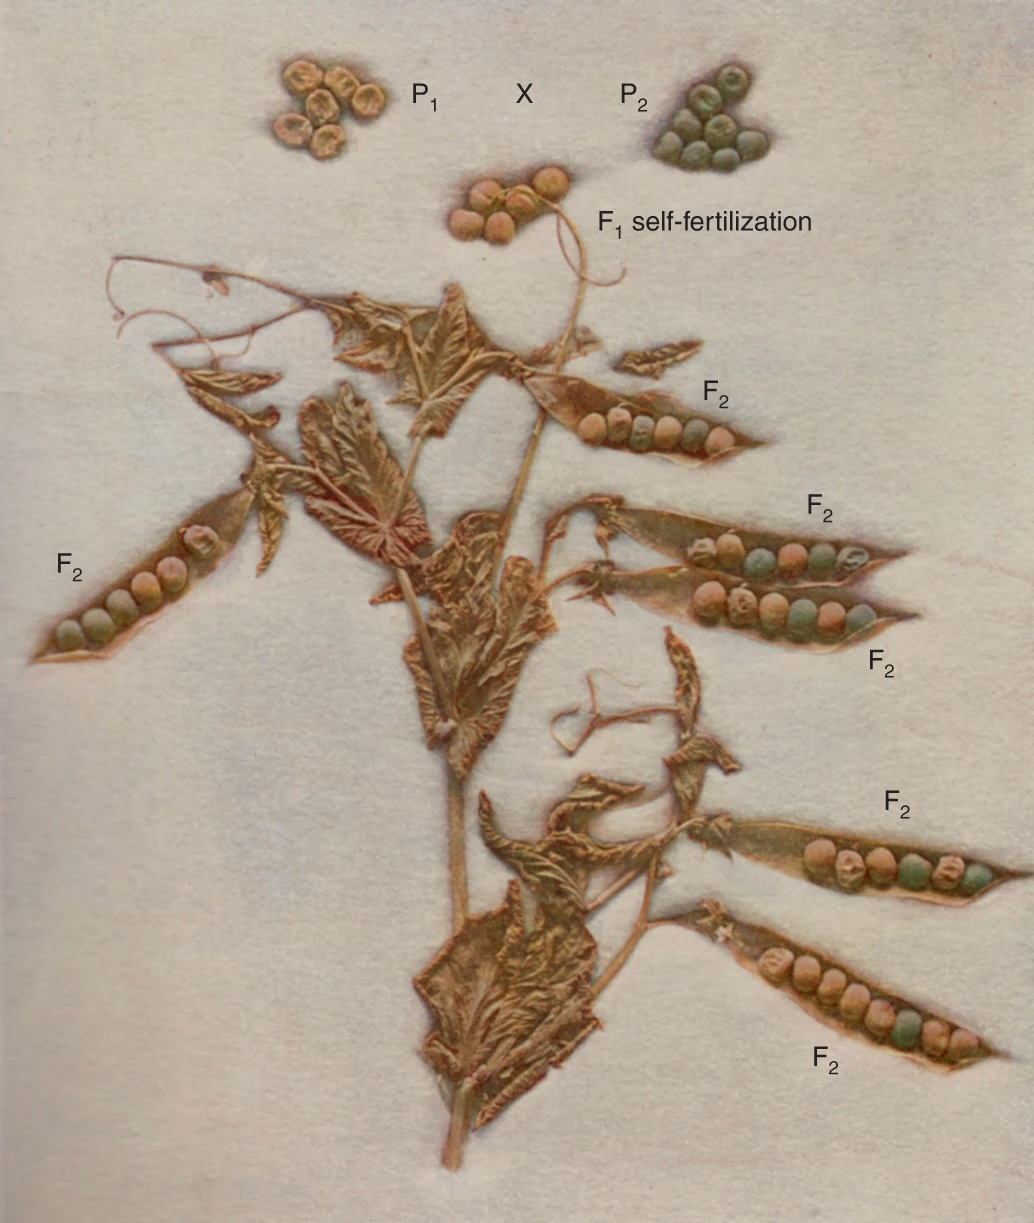
\includegraphics[keepaspectratio, width  =\textwidth]{img/crossedPeas}
			
		\end{column}
		\begin{column}{0.4\textwidth}
			\small	
			
			\textbf{The law of dominance: } for some traits, the presence of one kind of particle masks the presence of another.

			\vspace{10pt}
			
			How does the image demonstrate \textbf{the law of dominance}?  \pause
			
			\vspace{10pt}
			
			Answer: \textit{The uniformity of trait values in the F1 generation}
			
			
		\end{column}		
		
	\end{columns}
\end{frame}


\begin{frame}
	
	\frametitle{Mendel's Laws}
	\begin{columns}
		\begin{column}{0.6\textwidth}
			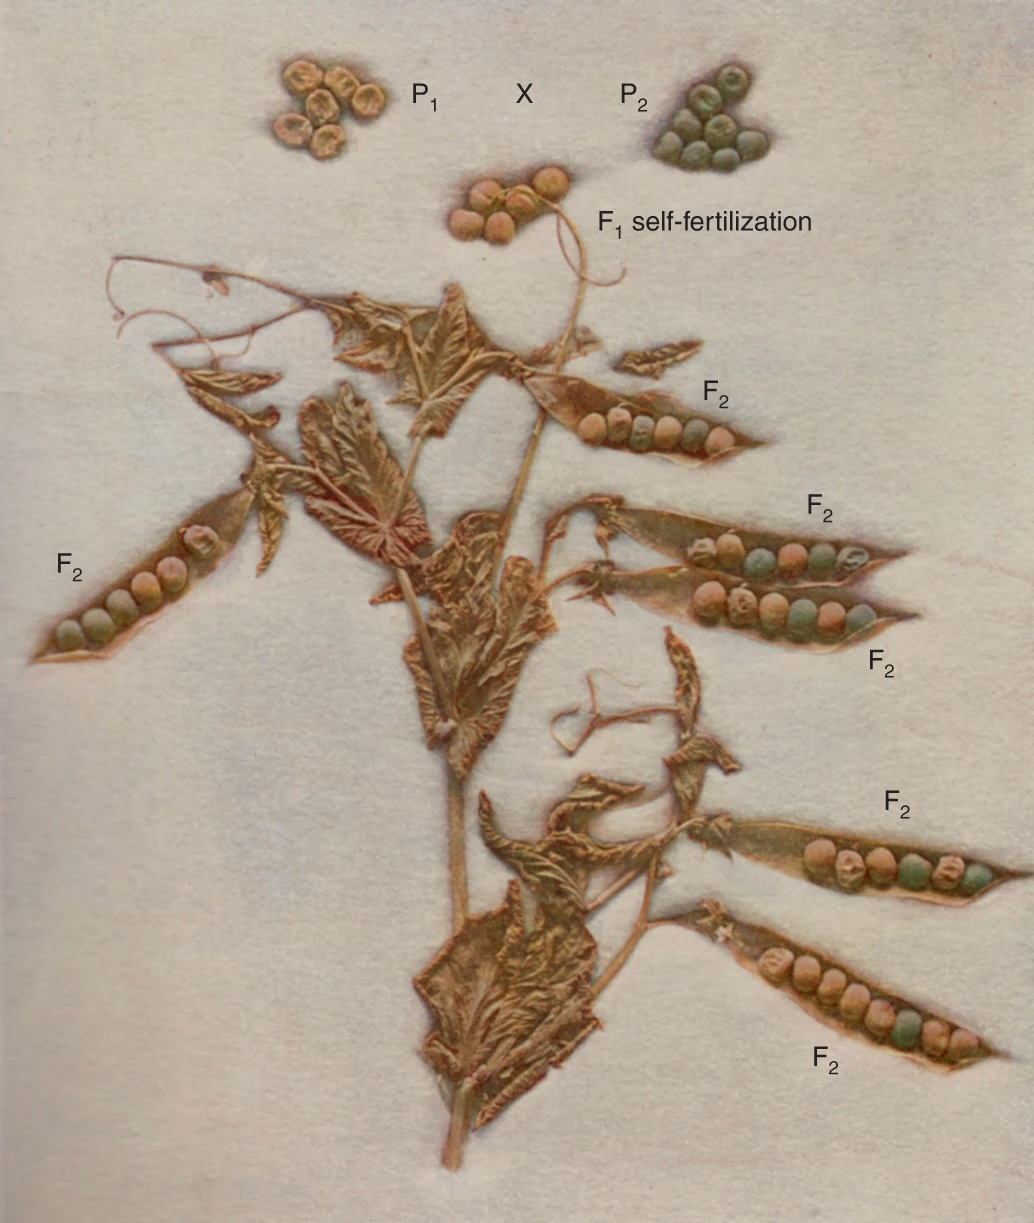
\includegraphics[keepaspectratio, width  =\textwidth]{img/crossedPeas}
			
		\end{column}
		\begin{column}{0.4\textwidth}
			\small	
			\textbf{The law of independant assortment:} when two individuals differ in more than two pairs of traits, the inheritance of one pair of traits is independent of another 
			\vspace{10pt}
			
			How does the image demonstrate \textbf{the law of  independant assortment}? \pause
			
			\vspace{10pt}
			
			Answer: \textit{The fact that wrinkly green peas and smooth yellow peas are seen in the F2 generation}			
			
			
		\end{column}		
		
	\end{columns}
\end{frame}




\begin{frame}
	
	\frametitle{Mendel's Laws}
	\begin{columns}
		\begin{column}{0.6\textwidth}
			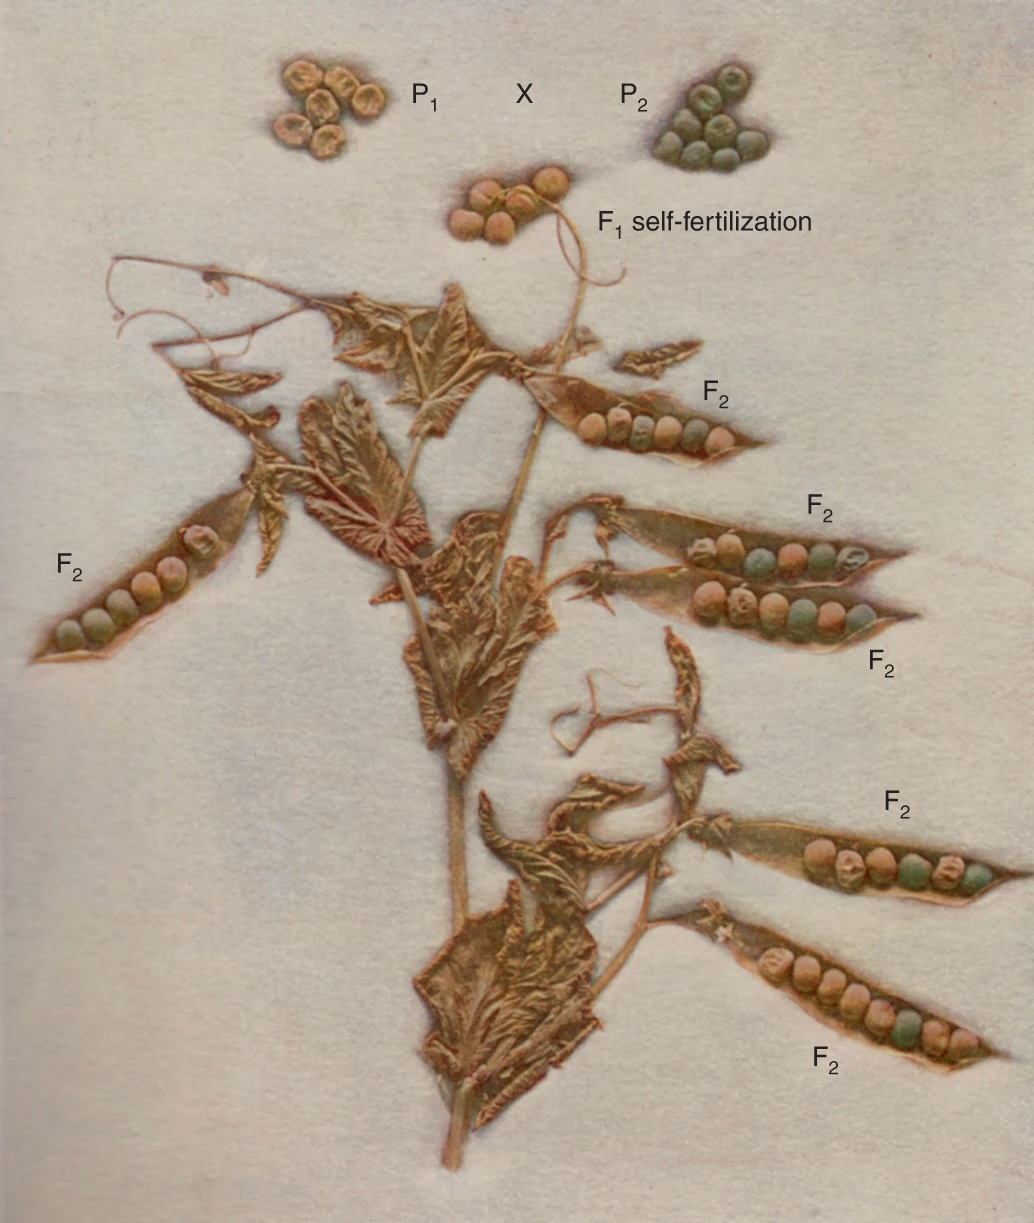
\includegraphics[keepaspectratio, width  =\textwidth]{img/crossedPeas}
			
		\end{column}
		\begin{column}{0.4\textwidth}
			\small	
		I count 38 F2 seeds \\
		\bigskip
		13 Green : 25 Yellow\\
		
		9 Wrinkly : 29 Smooth
		
			\vspace{10pt}
		Why do we see these ratios?
			
		\end{column}		
		
	\end{columns}
\end{frame}


\begin{frame}
	\frametitle{Mendelian Terminology}

	
	 Remember, Mendel crossed "true" green (\textbf{G}) peas with "true" yellow (\textbf{Y}) peas.

\bigskip

	The table below gives the results of the self-fertlization of the F1 generation\\
	
	\bigskip	
\begin{columns}	
	\begin{column}{0.5\textwidth}


\begin{tabular}{c|c|c|c|}
	\multicolumn{2}{c|}{} & \multicolumn{2}{c|}{\textbf{GY}} \\
	\multicolumn{2}{c|}{} & \textbf{G} & \textbf{Y} \\
	\hline 
	\multirow{2}{*}{\textbf{YG}}	& \textbf{G}& GG& YG \\		
	\cline{2-4} 
	&	\textbf{Y} & YG & YY \\
	\hline
\end{tabular}
	\end{column}

	\begin{column}{0.5\textwidth}

	
	\end{column}
	\end{columns}
	
	
\end{frame}




\begin{frame}
	\frametitle{Codominance}
	
	\begin{center}
		\newcommand{\picA}{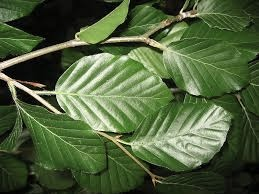
\includegraphics[keepaspectratio, height=2.25in,width=1.6in]{img/roundBeechLeaf}}
		\newcommand{\picB}{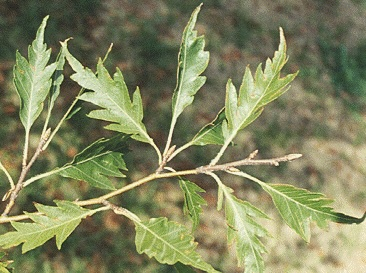
\includegraphics[keepaspectratio, height=2.25in,width=1.6in]{img/cutBeechLeaf}}
		\Huge
		\parbox{\widthof{\picA}}{\picA} $\times$ 
		\parbox{\widthof{\picB}}{\picB} 
	\end{center}	
	\normalsize
	A leaf shape trait controlled by a single gene 
	\bigskip
	
	Assuming the two individuals are homozygotes, how could you figure out if the allele for the cut leaf phenotype is dominant, recessive or codominant?
	
\end{frame}




%%%%%%%%

\begin{frame}
	\frametitle{Test Crosses}
	Leaf phenotypes in European beech, \textit{Fagus sylvatica}
	\begin{center}
	\newcommand{\picA}{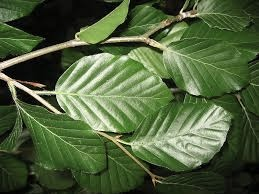
\includegraphics[keepaspectratio, height=2.25in,width=1.6in]{img/roundBeechLeaf}}
	\newcommand{\picB}{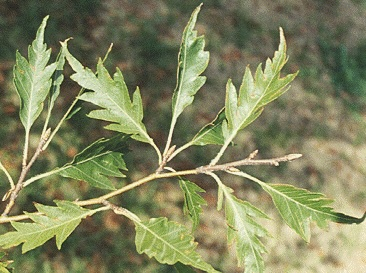
\includegraphics[keepaspectratio, height=2.25in,width=1.6in]{img/cutBeechLeaf}}
	\Huge
	\parbox{\widthof{\picA}}{\picA} $\times$ 
	\parbox{\widthof{\picB}}{\picB} 
\end{center}	
	\normalsize
	A leaf shape trait controlled by a single gene 
	\bigskip
	
	Assuming the two individuals are homozygotes, how could you figure out if the allele for the cut leaf phenotype is dominant, recessive or codominant?
	
\end{frame}





%%% Slide 13

\begin{frame}
	
	\frametitle{Particulate Inheritance and Classical Genetics}
	
	\begin{columns}[T]
		
		\begin{column}{0.6\textwidth}
			
			\begin{itemize}
				\item Proposed in 1865 and 1866
				\item 6-7 years after Darwin’s Theory of Evolution
				\item As far as anyone knows, Darwin was totally unaware of Mendel\textsuperscript{\textit{but see notes!}}
				\vspace{20pt}
				\item Represents the foundation of classical genetics
				\item \textbf{Classical genetics} refers to the study of genetic patterns observable from reproductive events
			\end{itemize}
			
			
		\end{column}
		\begin{column}{.4\textwidth}
			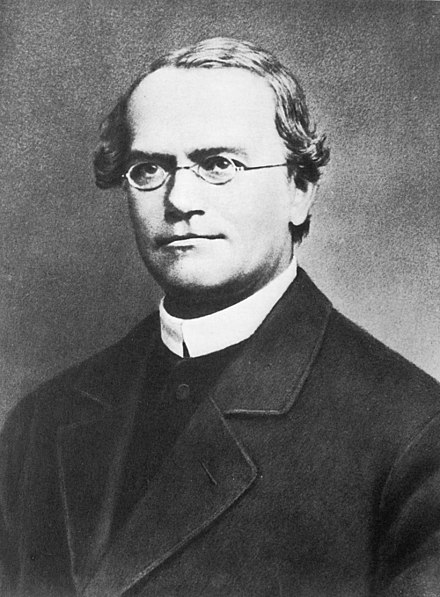
\includegraphics[keepaspectratio, width  =\textwidth]{img/mendel}
			\centering
			More peas please
		\end{column}
		
		\note{Pea pic from: \url{https://www.thoughtco.com/domestication-history-of-peas-169376}}
		
		
	\end{columns}
	\note{
		A letter from Darwin to Alfred Russel Wallace - 6th Februrary 1866
		
		``My dear Wallace,
		
		After I had despatched my last note, the simple explanation which you give had occurred to me, and seems satisfactory.
		
		I do not think you understand what I mean by the non-blending of certain varieties. It does not refer to fertility; an instance will explain; I crossed the Painted Lady and Purple sweet-peas, which are very differently coloured vars, and got, even out of the same pod, both varieties perfect but none intermediate. Something of this kind I shd. think must occur at first with your butterflies got the 3 forms of Lythrum; tho’ these cases are in appearance so wonderful, I do not know that they are really more so than every female in the world producing distinct male got female offspring.
		
		I am heartily glad that you mean to go on preparing your journal.6
		
		Believe me yours,  very sincerely,
		
		Ch. Darwin"}
		
\end{frame}







%%% Slide 14


\begin{frame}
	\frametitle{Reconciling the Mendelians and the Biometricians}
	
\small	Mendel's results went largely unnoticed in his lifetime,  but they were rediscovered and publicised in the early 1900s
	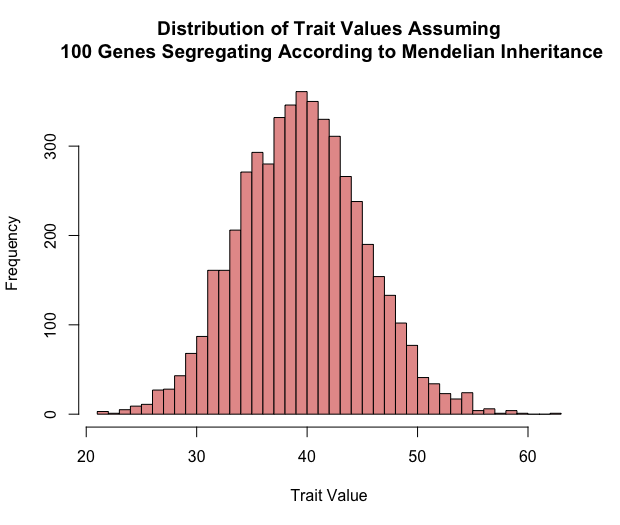
\includegraphics[keepaspectratio, width  =0.5\textwidth]{img/100Genes}
\end{frame}





\begin{frame}
	\frametitle{Reconciling the Mendelians and the Biometricians}

				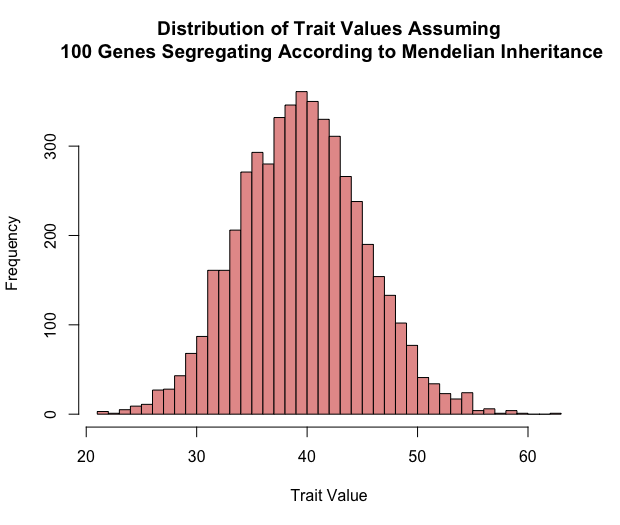
\includegraphics[keepaspectratio, width  =\textwidth]{img/100Genes}
\end{frame}

%%% Slide 13

\begin{frame}
	
	\frametitle{Branches of Genetics}
	
	\begin{columns}[T]
		
		\begin{column}{0.45\textwidth}
			\begin{itemize}
			\item{Behavioural genetics}
			\item{\textbf{Classical genetics}}
			\item{Developmental genetics}
			\item{\textbf{Conservation genetics}}
			\item{\textbf{Ecological genetics}}
			\item{\textbf{Evolutionary genetics}}
			\item{\textbf{Genecology}}
			\item{Genetic engineering}
			\item{Genomics}
			
			\end{itemize}
			
		\end{column}
		\begin{column}{.45\textwidth}
			\begin{itemize}
			\item{Medical genetics}
				\item{Forensics}
				\item{Molecular genetics}
				\item{\textbf{Quantitative genetics}}
				\item{\textbf{Population genetics}}
				\item{Phylogenetics}
				\item{Statistical genetics}
				\item{Genetic epidemiology}
				\item{Archaeogenetics}
			\end{itemize}
		\end{column}
		\end{columns}
		\blfootnote{A non-complete and \textit{slightly} biased list}
\end{frame}

%%% Slide 15

\begin{frame}[fragile]
	\frametitle{Extra Material}
	
	\textbf{Below is the R code to make the figures on the infinitesimal model - feel free to play around with it}
	\begin{adjustbox}{max width=\textwidth}
		
	\begin{lstlisting}[language=R]

# Demonstrate the distribution of trait values for a quantitative trait
# Under Mendelian segregation for an arbitrary number of genes
# Assumes random mating, constant effect sizes, constant allele frequencies
	
nGenes = 100
alleleFrequency = 0.2
popSize = 5000
effectSize = 1
			
hist( 
	replicate(popSize,
		sum(  1 * rbinom(nGenes, 2, alleleFrequency) ) ),
	col = "#e69b99",
	xlab=  "Trait Value",
	main= paste("Distribution of Trait Values in F2s Assuming\n",nGenes, 
		"Genes Segregating According to Mendelian Inheritance"),
	breaks = 40)
		\end{lstlisting}
\end{adjustbox}
\end{frame}


%%% Slide 17
\end{document}

The Mendelian Biometrician debate was rather fierce. ``Mr. Bateson devotes many words to these questions, but one cannot help feeling that his speculations would have had more value had he kept his emotions under better control; the style and method of the religious revivalist are ill-suited to scientific controversy. It is difficult to speak with patience either of the turgid and bombastic preface to 'Mendel’s Principles,' with its reference to Scribes and Pharisees, and its Carlylean inversions of sentence, or of the grossly and gratuitously offensive reply to Professor Weldon and the almost equally offensive adulation of Mr. Galton and Professor Pearson  Yule 1990}



